\documentclass{article}

% Math packages
\usepackage{amsthm, amssymb, enumitem}

% Margins settings
\usepackage[margin=1.2in]{geometry}

% Bracket notation (quantum computing/information)
\usepackage{tikz}
\usetikzlibrary{quantikz}
\usepackage{braket}

% Spacing
\usepackage{parskip}
\usepackage{centernot}

% Required for inserting images
\usepackage{graphicx}
\graphicspath{{./Figures/}}

% Hyperlinks
\usepackage[colorlinks=true, allcolors=blue]{hyperref}

% Header
\usepackage{fancyhdr}
\pagestyle{fancy}
\lhead{November 4th, 2024}
\chead{Optimization for Data Science}
\rhead{University of Waterloo}

% Custom commands
\newcommand{\R}{\mathbb{R}}             % real numbers
\newcommand{\E}{\text{E}}               % expectation
\newcommand{\x}{\vec{x}}
\newcommand{\dom}{\text{dom}}           % domain
\newcommand{\relint}{\text{relint}}     % relative interior
\newcommand{\ds}{\displaystyle}
\newcommand{\indep}{\perp\!\!\!\perp}

\setlength\parindent{0pt}

\title{CO 673/CS 794 - Optimization for Data Science\\Lecture 16 Notes}
\author{University of Waterloo}
\date{November 4th, 2024, 11h30-12h50 in MC 2054}

\begin{document}

\maketitle

\section{Administration}

\begin{itemize}
    \item Problem set 5 to be posted on Wednesday
\end{itemize}

Recall from the previous lecture: the subgradient inequality. But if $f$ is not differentiable, we can still have linear underestimators.

\begin{center}
    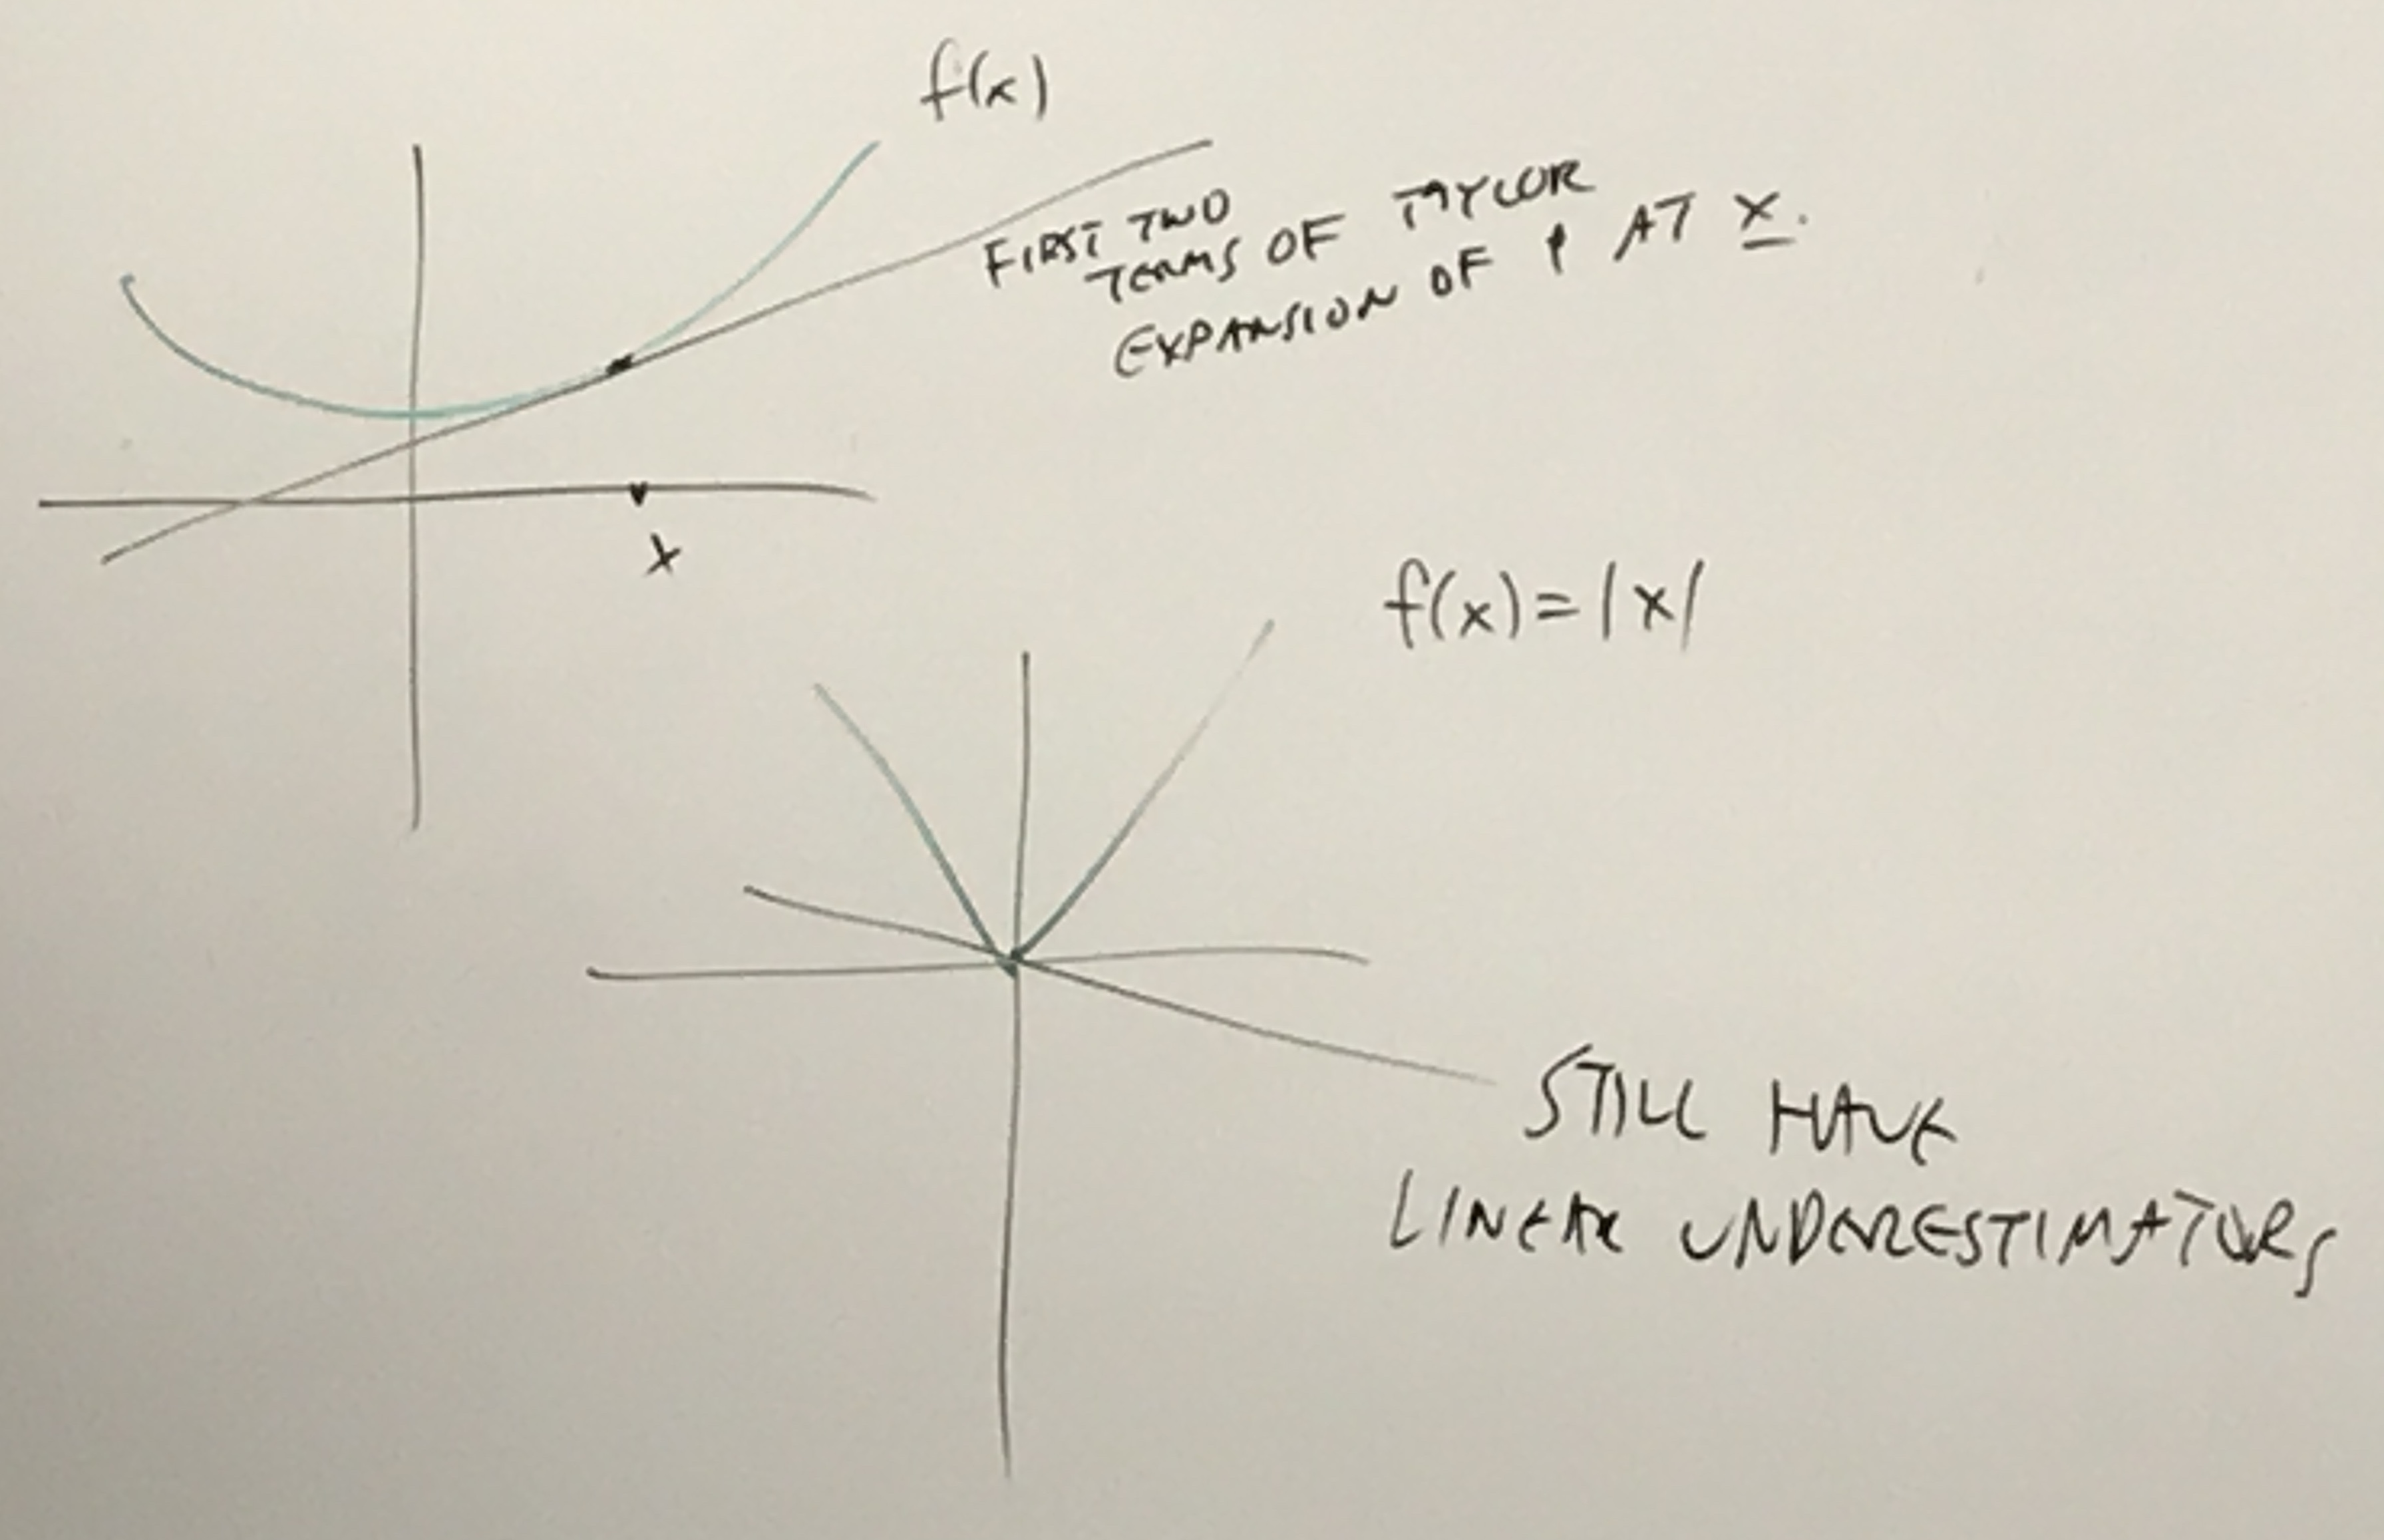
\includegraphics[scale=0.1]{subgrad_ineq.JPG}
\end{center}

Given $f \colon \R^n \to \R \cup \{\infty\}$ and given $\x \in \dom(f)$, we say that $\vec{g} \in \R^n$ is a \textbf{subgradient} of $f$ at $\x$ if $\forall \vec{y} \in \R^n$,
\[
    f(\vec{y}) \geq f(\x) + \vec{g}^\top(\vec{y} - \x)
\]

The subdifferential of $f$ at $\x$, denoted $\partial f(\x)$ is the set of all subgradients of $f$ at $\x$.

\textbf{Theorem} (Chapter 8) \textit{Let $f \colon \R^n \to \R \cup \{\infty\}$ be convex. Then,}
\begin{enumerate}
    \item \textit{$\forall \x \in \dom(f)$, $\partial f(\x)$ is closed and convex.}

    \textit{Recall: $\dom(f) = \{\x : f(\x) < \infty\}$ for convex functions $f$. $\dom(f)$ is a convex set.}

    \item \textit{If $\x \in \underbrace{\relint}_{\text{relative interior}}(\dom(f))$ then $\partial f(\x) \neq \varnothing$.}
    \item \textit{If $\x \in \dom(f)^\circ$, then $\partial f(\x)$ is bounded, hence compact.}
    \item \textit{$\forall \x \in \dom(f)^\circ$, then
    \[
        f \text{ is differentiable at } \x \iff \partial f(\x) = \{\nabla f(\x)\}
    \]}
\end{enumerate}

Recall: an affine set is a solution set to a system of linear equations.

Given $C \subseteq \R^n$, the \textbf{affine hull}, $\text{aff}(C)$ is the smallest affine set containint $C$, i.e., common intersection of all affine sets containing $C$.

The relative interior of $C$, $\relint(C)$ is the interior of $C$ with respect to the topology of $\text{aff}(C)$, i.e.,
\[
    \relint(C) = \{\x \in C : \exists r > 0 \text{ such that } B_r(\x) \underbrace{\cap\, \text{aff}(C)}_{\text{\tiny if omitted, same def. as int.}} \subseteq C \}
\]

\begin{center}
    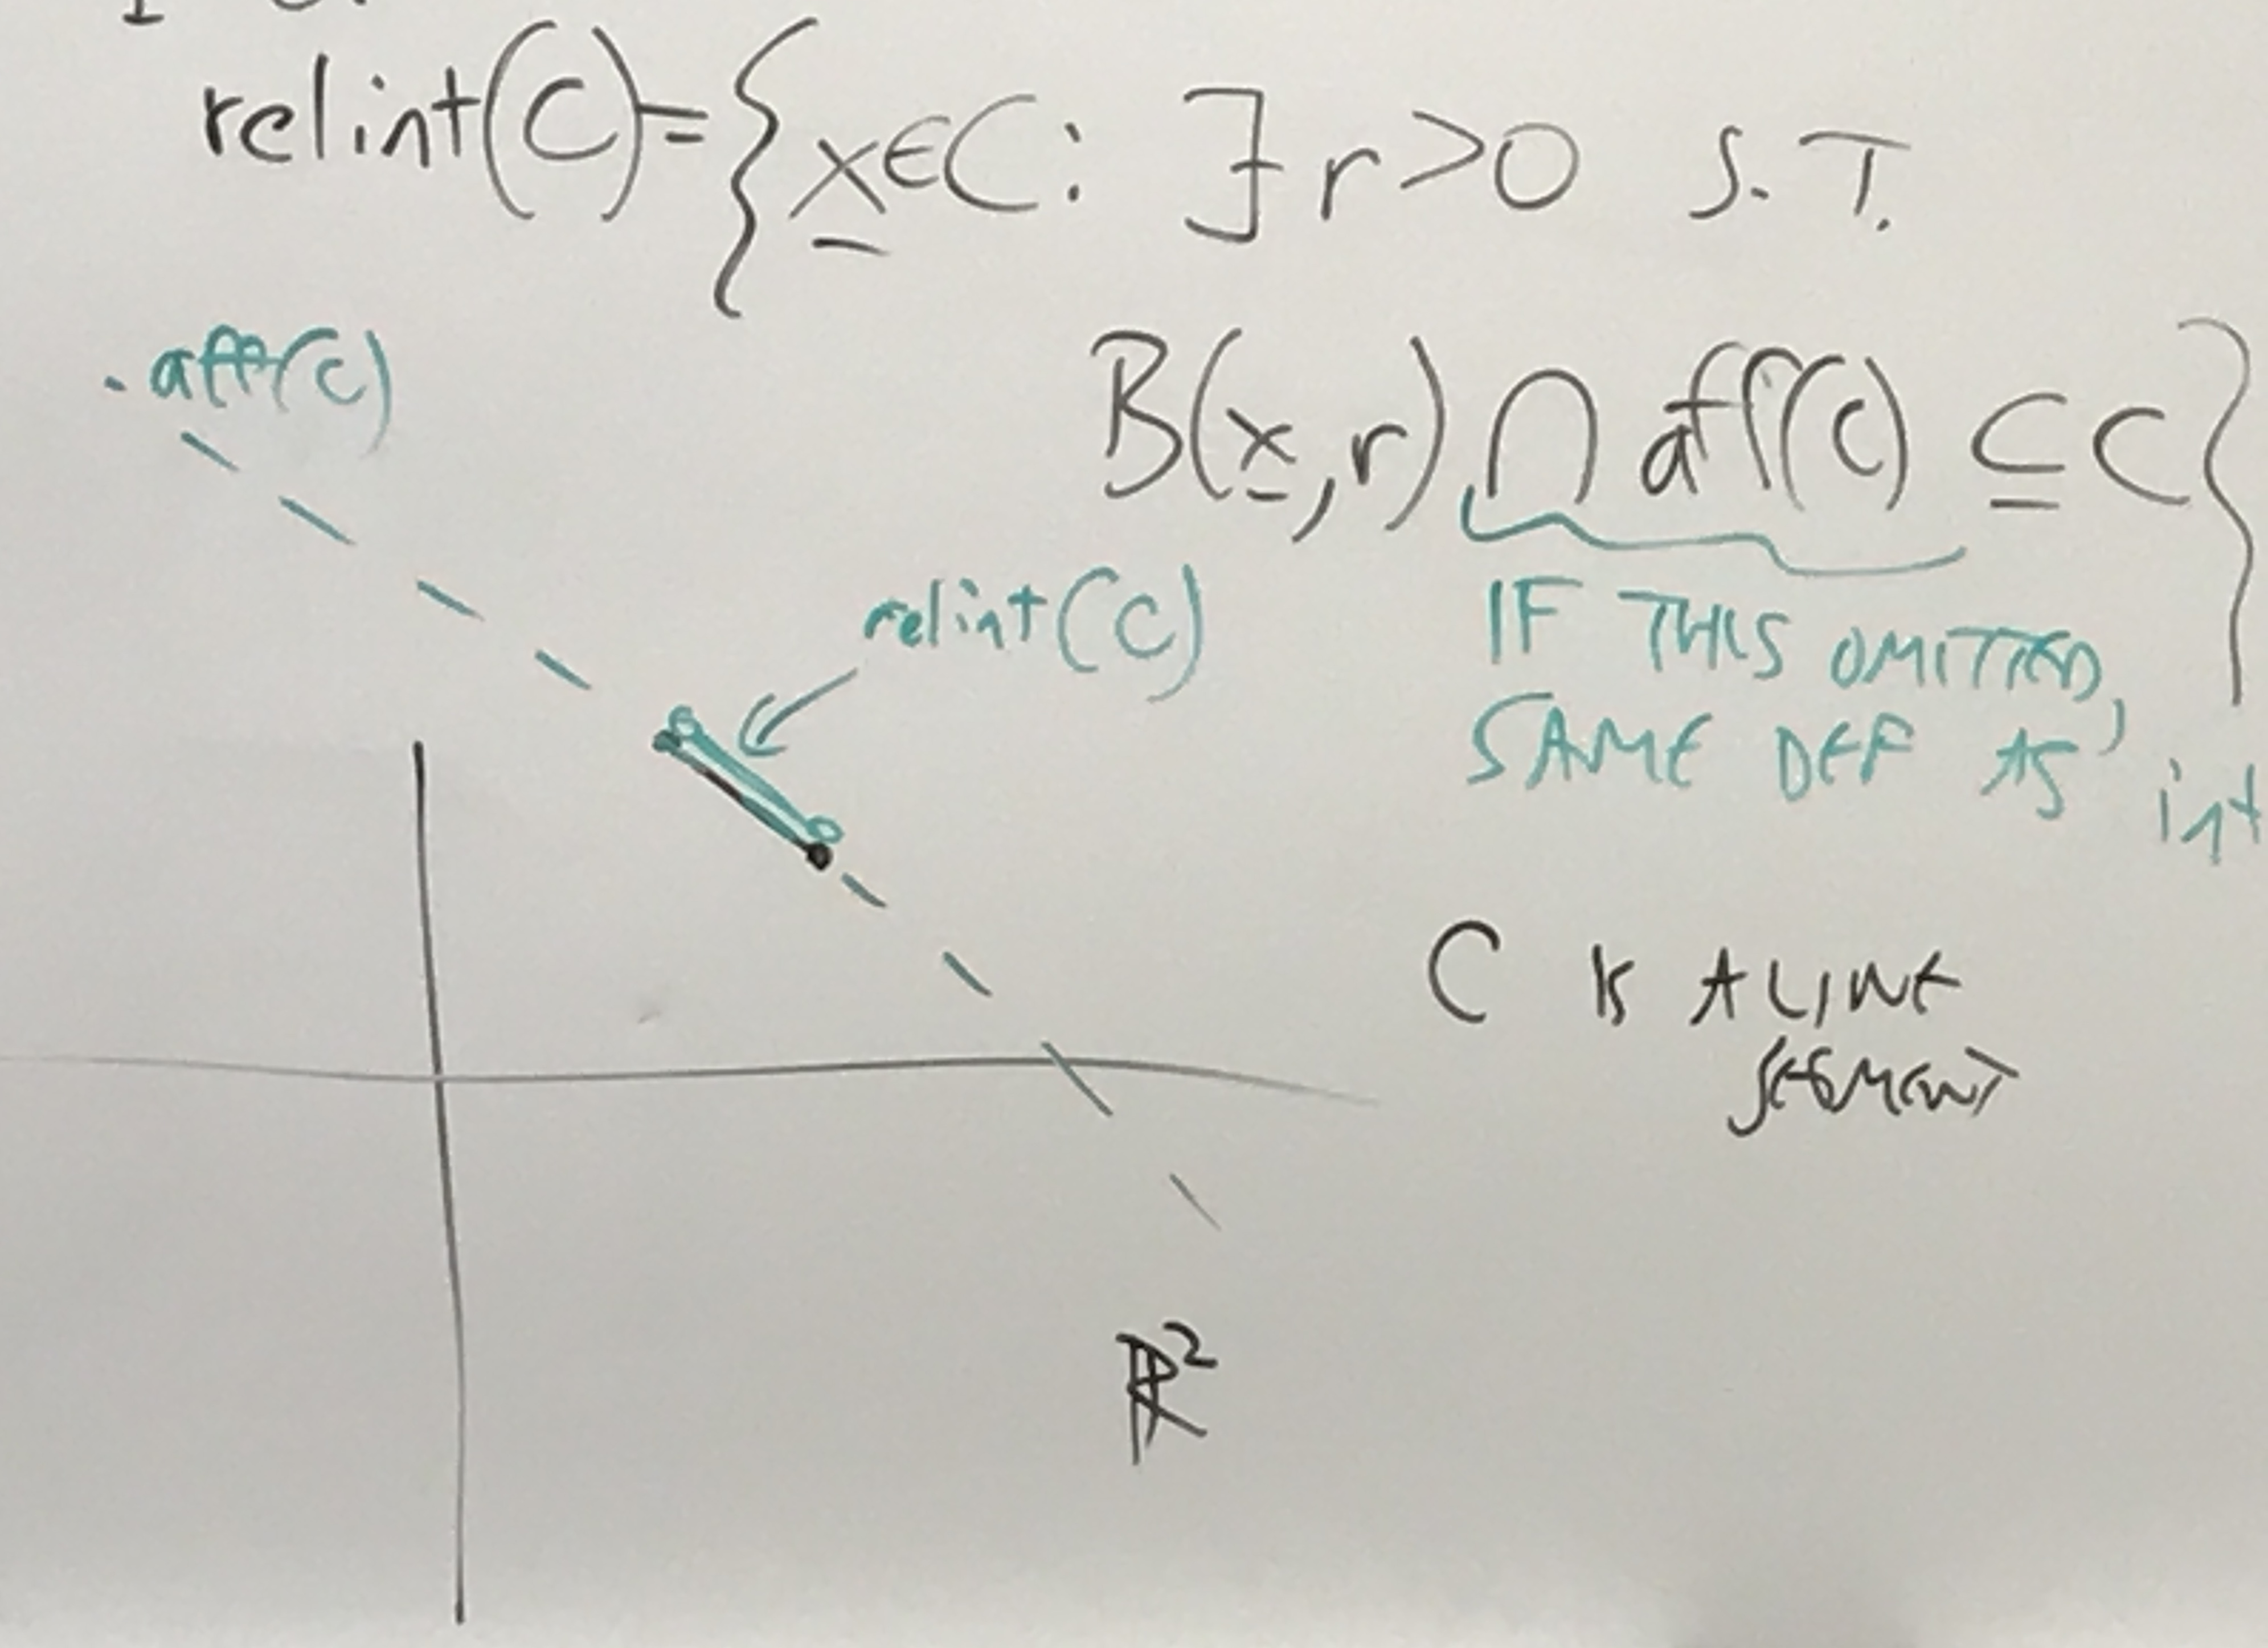
\includegraphics[scale=0.08]{affine_set.JPG}
\end{center}

\textbf{Theorem.} \textit{If $C \subseteq \R^n$ is convex and non-empty, then $\relint(C) \neq \varnothing$.}

\begin{center}
    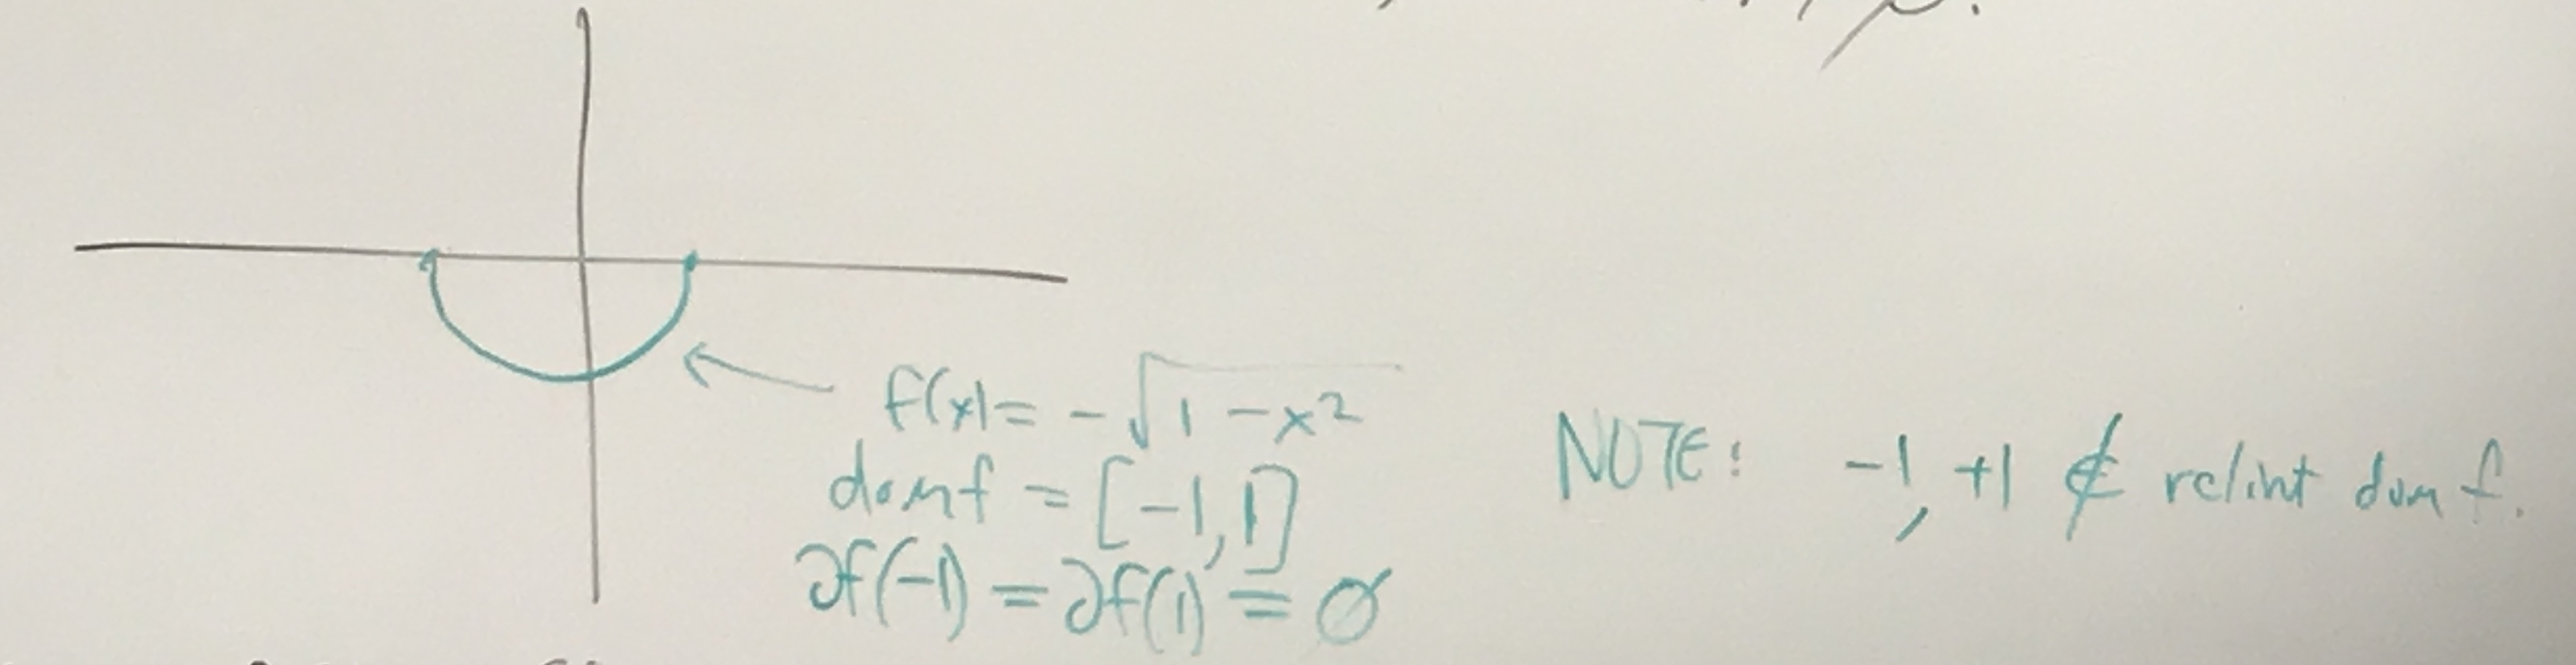
\includegraphics[scale=0.1]{relative_interior.JPG}
\end{center}

Suppose that
\[
    f(\x) = \begin{cases}
        0, & \text{if } \x \in [0;\; 1] \\
        \infty, & \text{if } \x \notin [0;\; 1]
    \end{cases}
\]
This is the indicator function of the set $[0;\; 1]$.

If $C \subseteq \R^n$ is a convex set, then,
\[
    I_c(\x) = \begin{cases}
        0, & \text{if } \x \in C \\
        \infty, & \text{if } \x \notin C
    \end{cases}
\]
is convex.

Indicator functions of convex sets are convex functions.

\textit{Claim.} $\partial f(1) = [0;\; \infty)$.

\begin{center}
    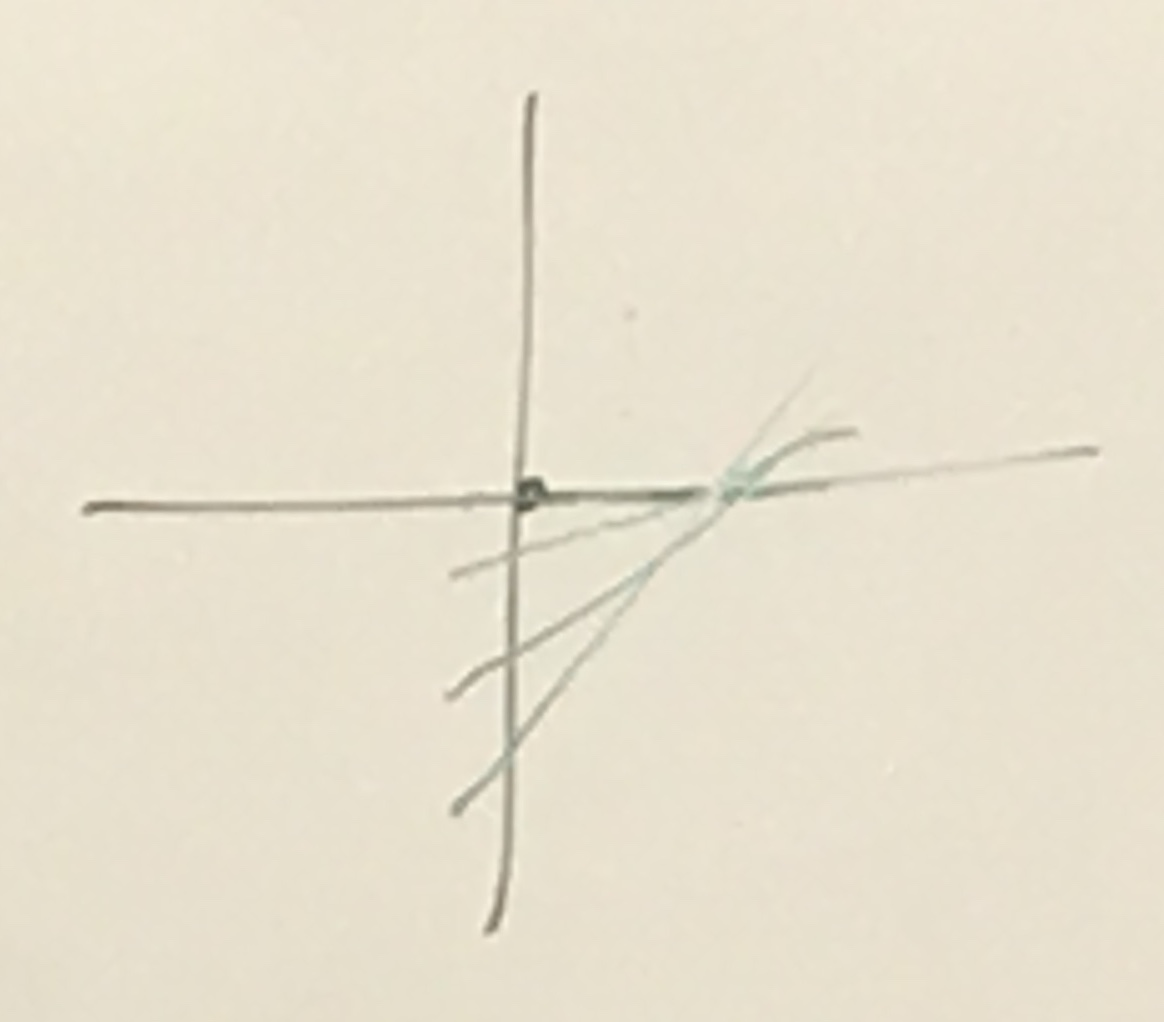
\includegraphics[scale=0.2]{indicator.JPG}
\end{center}

\begin{proof}
    \begin{itemize}
        \item $[0;\; \infty) \subseteq \partial f(1)$:

        i.e., $\forall g \geq 0,\, y \in \R$, $f(y) \geq 0 + g(y - x)$, where $x = 1$.

        Cases:
        \begin{itemize}
            \item $y > 1$: $f(y) = \infty$, trivially true.
            \item $y \in [0;\; 1]$: $0 \geq \text{ non-positive}$, OK.
            \item $y < 0$: trivial.
        \end{itemize}

        \item $\partial f(1) \subseteq [0;\; \infty)$:

        \[
            f(y) \overset{\text{?}}{\geq} f(x) + g(y - x), \quad \text{for } x = 1,\, \forall y.
        \]
        We take $y = 0$. Since the following inequality is false if $g < 0$:
        \[
            0 \underbrace{\geq}_{\text{FALSE if } g < 0} 0 + g(0 - 1)
        \]
        we have that $g < 0 \implies g \notin \partial f(1)$
    \end{itemize}
\end{proof}

\textit{Claim.} For $f(x) = |x|$,

\[
    \partial f(x) = \begin{cases}
        \{1\}, & \text{if } x > 0 \\
        [-1;\; 1], & \text{if } x = 0 \\
        \{-1\}, & \text{if } x < 0
    \end{cases}
\]

% IMAGE of |x|

$f \colon \R^n \to \R \cup \{\infty\}$ is proper if $\dom(f) \neq \varnothing$.

$f \colon \R^n \to \R \cup \{\infty\}$ is closed if epi$f$ is a closed set, where epi$f = \{(\vec{x},\, y) \in \R^n \times R: y \geq f(x)\}$.

$\dom(f)$ is closed $\iff$ epi$f$ is closed.

\begin{center}
    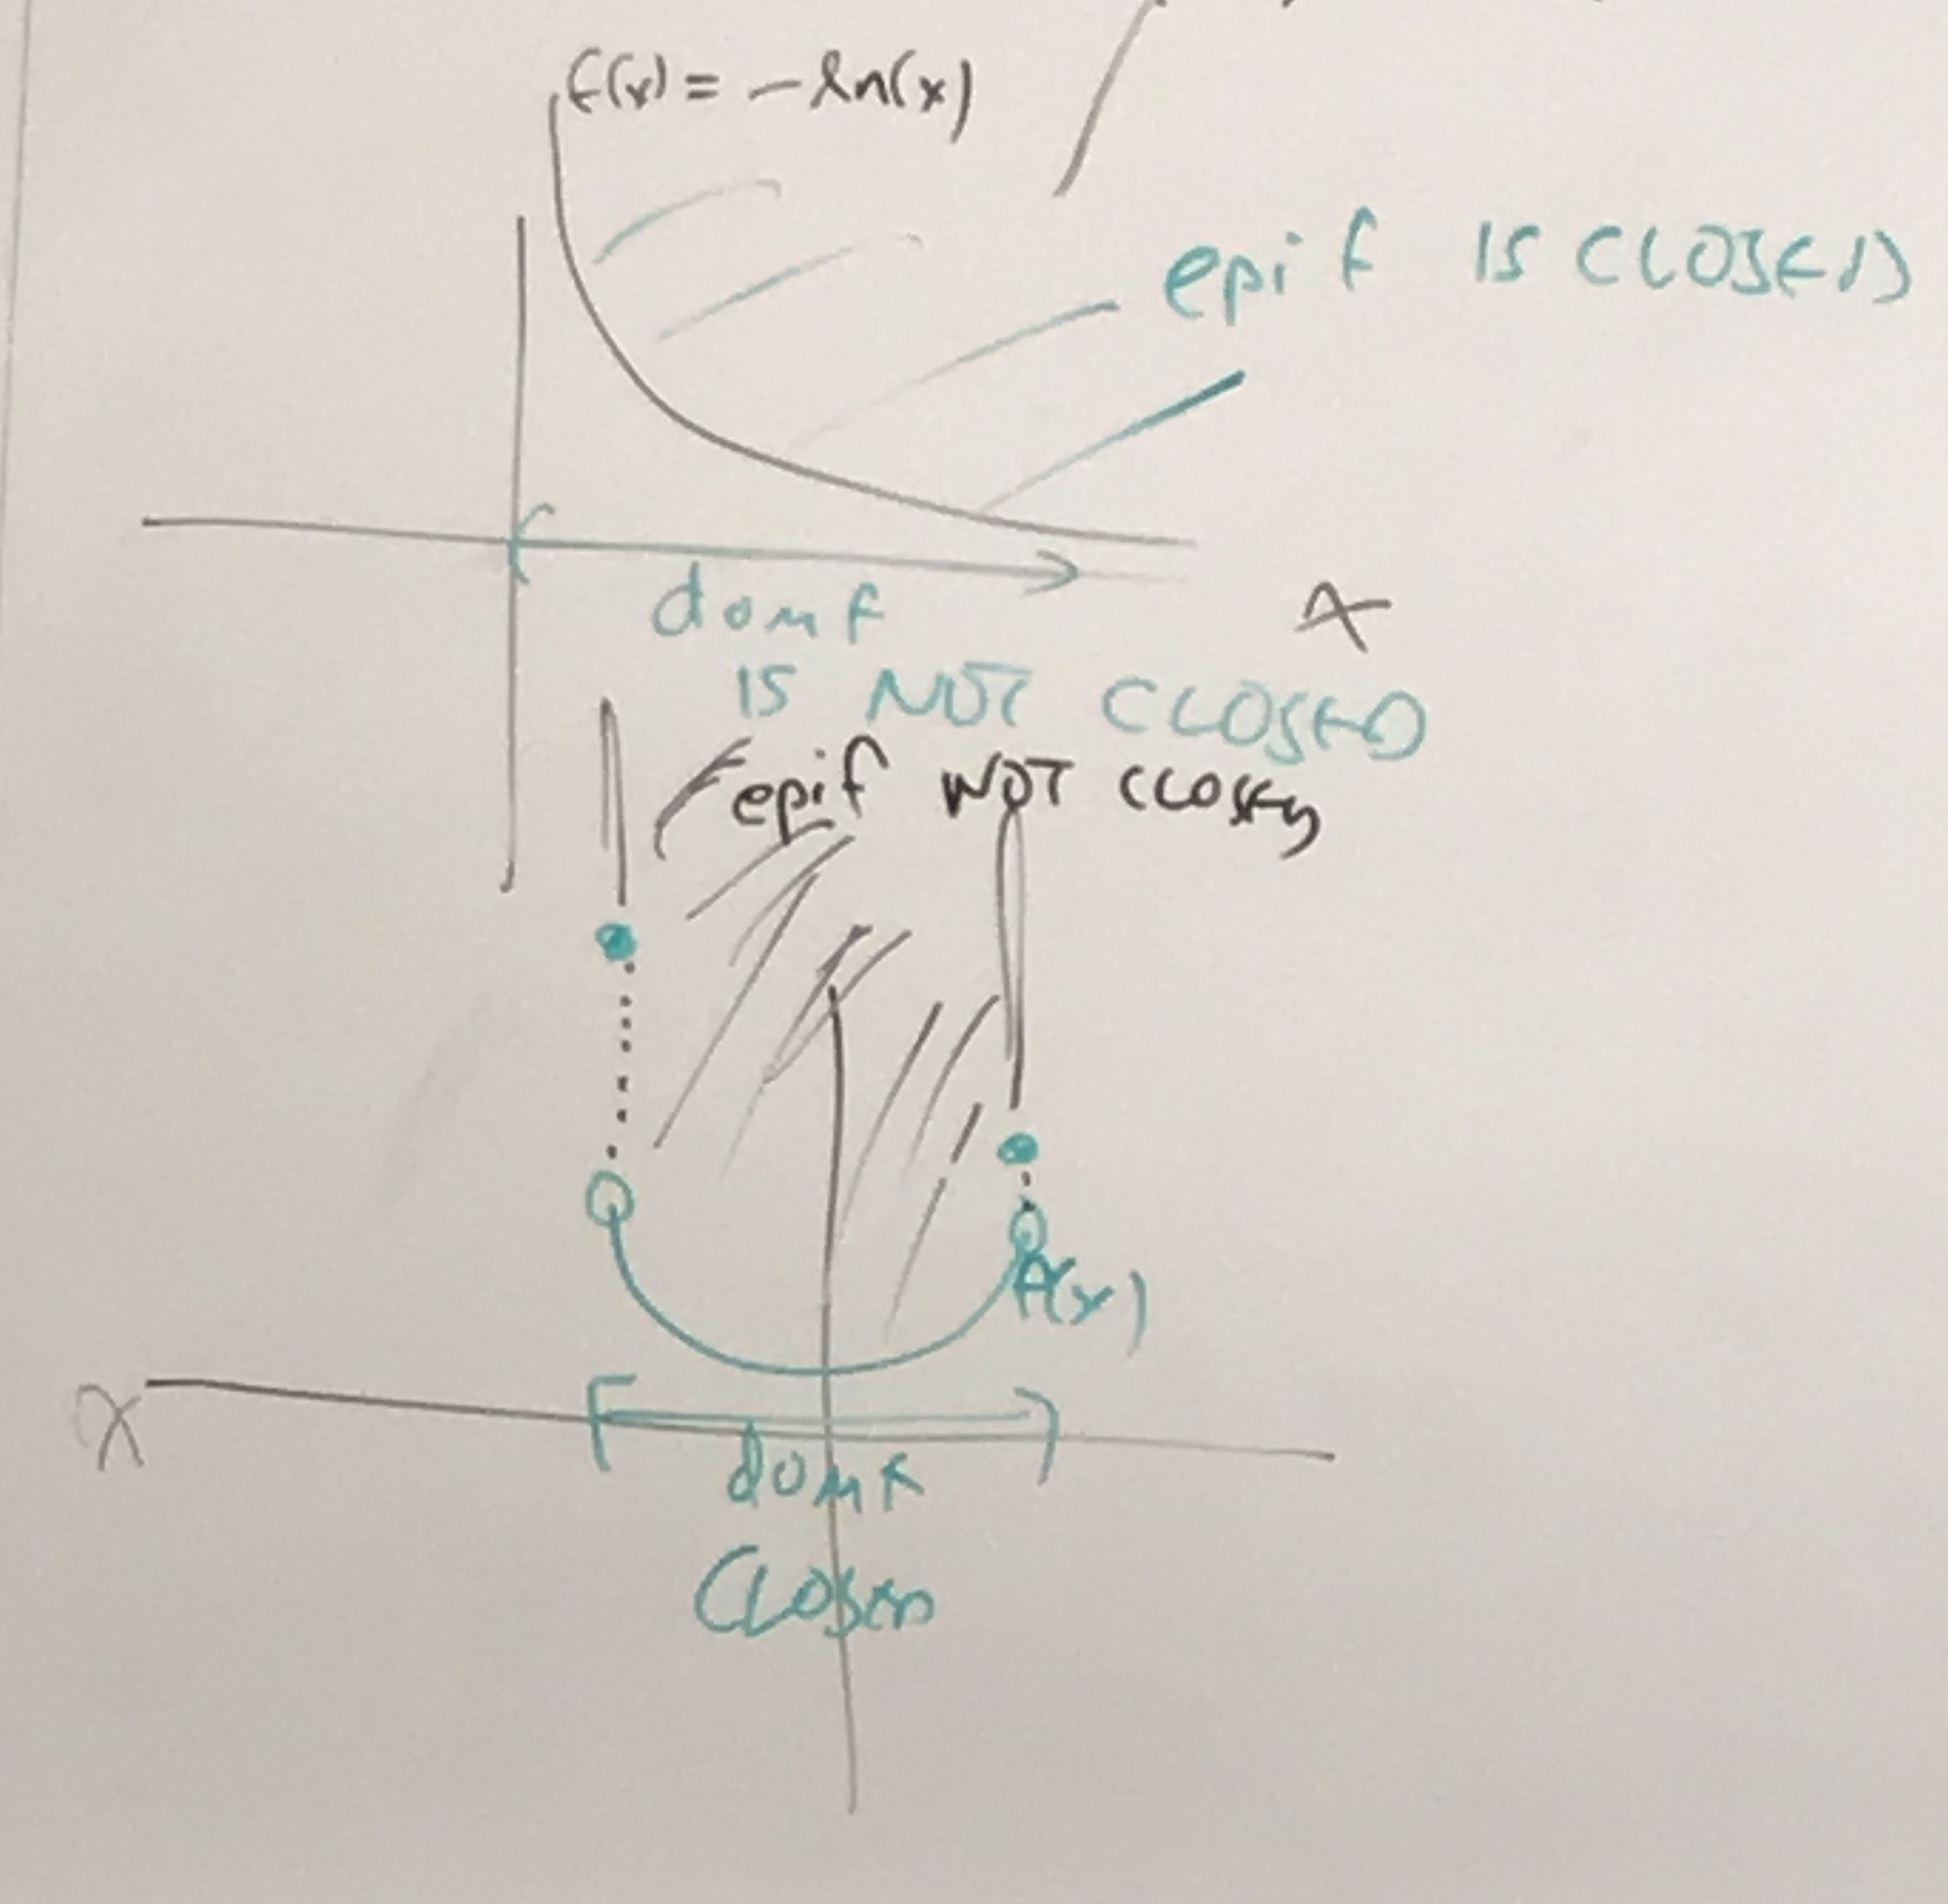
\includegraphics[scale=0.1]{epif.JPG}
\end{center}

\textbf{Theorem.}

For convex function $f \colon \R^n \to \R \cup \{\infty\}$. $f$ is closed $\iff \forall \beta \in \R$, the level set $\{x : f(x) \leq \beta\}$ is closed (could be empty).

For convex functions $f$ and $g$
\[
    f \text{ and } g \text{ closed} \iff f + g \text{ closed}
\]

\textbf{Theorem.} (Like Theorem 8.11 but much more general)

Suppose that $f$ and $g$ are convex functions. Suppose that $\underbrace{\relint(\dom(f)) \cap \relint(\dom(g)) \neq \varnothing}_{\text{a kind of C.Q.}}$.

Then, $\forall \x \in \dom(f) \cap \dom(g)$, $\partial (f + g)(\x) = \underbrace{\partial f(\x) + \partial g(\x)}_{\text{Minkkowski sum}}$.

\textbf{Theorem.} (in textbok)

$f \colon \R^n \to \R \cup \{\infty\}$ is minimized over $\R^n$ at $\x^* \in \dom(f) \iff 0 \in \partial f(\x^*)$.

Recall that a differentiable function $f \colon \R^n \to \R$ is minimized at $\x^* \iff \nabla f(\x^*) = \vec{0}$.

\begin{proof}
    \begin{align*}
        f \text{ is minimized at } \x^* &\iff \forall \vec{y} \in \R^n,\, f(\vec{y}) \geq f(\x^*) \\
        &\iff \forall \vec{y} \in \R^n,\, f(\vec{y}) \geq f(\x^*) + \vec{0}^\top(\vec{y} - \x^*) \\
        &\iff \vec{0} \in \partial f(\x^*)
    \end{align*}
\end{proof}

\textbf{Theorem (8.14).} If $\Omega \subseteq \R^n$ is closed, convex, and non-empty, then $I_\Omega$ is proper, closed, and convex.
\[
    \partial I_\Omega(\x) = \text{N}_\Omega(\x)
\]
Suppose that $f \colon \R^n \to \R \cup \{\infty\}$, then $f$ is differentiable on an open set containing $\Omega$, which is a non-empty, closed, convex set.

\begin{align*}
    f \text{ is minimized over } \Omega \text{ at } \x^* \in \Omega &\iff f + I_\Omega \text{ is minimized over } \R^n \\
    &\iff \vec{0} \in \partial(f + I_\Omega)(\x^*) \tag{by previous theorem} \\
    &\iff \vec{0} \in \partial f(\x^*) + \partial I_\Omega(\x^*) \tag{C.Q. holds} \\
    &\iff \vec{0} \in \{\nabla f(\x^*)\} + \partial I_\Omega(\x^*) \\
    &\iff \vec{0} \in \{\nabla f(\x^*)\} + \text{N}_\Omega(\x^*) \\
    &\iff -\nabla f(\x^*) \subseteq \text{N}_\Omega(\x^*) \tag{new proof of earlier theorem}
\end{align*}

\section{Minimization of composite functions (section 8.5 + Pset 5)}

\[
    \min(F(\x)) := f(\x) + \psi(\x)
\]
where $f \colon \R^n \to \R$ is $L$-smooth and convex, and $\psi$ is proper, closed, and convex. SVM-9 and $\ell_1$-LS.

\textbf{Theorem (8.16).} $F$ is minimized at $\x^* \iff -\nabla f(\x^*) \in \partial \psi(\x^*)$.

\begin{proof}
    $\partial F(\x^*) = \{\nabla f(\x^*)\} \partial \psi(\x^*)$.

    Note, the book imposes the additional, unnecessary, restriction that $\dom(f) = \R^n$.
\end{proof}

\textbf{Theorem (8.17).} $F$ is as above, additionally, assume that $f$ is $m$-strongly convex $(m > 0)$. Then, $F$ has a unique minimizer.

\begin{proof}
    Uniqueness:
    \begin{align*}
        f \text{ is strongly convex} &\implies F \text{ is strongly convex} \\
        &\implies F \text{ is strictly convex} \\
        &\implies \text{if } f \text{ has a minimizer, then it is unique.}
    \end{align*}
    Existence:

    $\forall \x \in \dom(\psi)$, the set $S_{\x_0} := \{\x \in \R^n : F(\x) \leq F(\x_0)\}$ is closed. This follows from: $\psi$ being closed by assumption, and $f$ being closed, $(\dom(f) = \R^n)$. These imply that $f + \psi$ is closed, and thus all level sets of $f + \psi$ are closed.

    Let $\x_0 \in \underbrace{\relint(\dom(\psi))}_{\text{non-empty since } \psi \text{ is proper, so } \dom(\psi) \neq \varnothing}$. Let $S = S_{\x_0}$ (we already know that $S$ is closed).

    \textit{Claim.} $S$ is bounded, choose $g \in \partial \psi(\x_0)$, which is non-empty by choice of $\x_0$.

    By the definition of the subgradient:
    \[
        \psi(\x) \geq \psi(\x_0) + \vec{g}^\top(\x - \x_0)
    \]
    By the strong subgradient inquality:
    \[
        f(\x) \geq f(\x_0) + \nabla f(\x_0)^\top(\x - \x_0) + \frac{m}{2}\|\x - \x_0\|^2
    \]
    We add:
    \[
        \forall \x \in \R^n,\, F(\x) \geq F(\x_0) + (g + \nabla f(\x_0))^\top(\x - \x_0) + \frac{m}{2}\|\x - \x_0\|^2
    \]
    Let $\x \in S$:
    \begin{align*}
        0 &\overset{\text{def. of } S}{\geq} F(\x) - F(\x_0) \\
        &\overset{\text{above ineq.}}{\geq} (\vec{g} + \nabla f(\x_0))^\top(x - \x_0) + \frac{m}{2}\|\x - \x_0\|^2 \\
        &\overset{\text{C-S}}{\geq} -\|g + \nabla f(\x_0)\| \cdot \|\x - \x_0\| + \frac{m}{2}\|\x - \x_0\|^2
    \end{align*}
    Divide by $\|\x - \x_0\|$:
    \begin{align*}
        &\implies \quad 0 \geq -\|\vec{g} + \nabla f(\x_0)\| + \frac{m}{2}\|\x - \x_0\| \\
        &\implies \quad \forall \x \in S,\, \|\x - \x_0\| \leq \frac{2}{m}\|\vec{g} + \nabla f(\x_0)\| \\
        &\implies \quad S \subseteq B_r(\x_0),\, \text{where } r = \frac{2}{m}\|\vec{g} + \nabla f(\x_0)\|
    \end{align*}
    So, $S$ is compact an non-empty.

    $\forall \x \in S$, $F(\vec{y}) \leq F(\x_0)$. $F$ is also bounded below on $S$:
    \begin{align*}
        F(\x) &\geq F(\x_0) + (g + \nabla f(\x_0))^\top(\x - \x_0) \\
        &\overset{\text{C-S}}{\geq} F(\x_0) - \|\vec{g} + \nabla f(\x_0)\| \cdot \underbrace{\|\x - \x_0\|}_{\leq \frac{2}{m}\|\vec{g} + \nabla f(\x_0)\|} \\
        &\geq F(\x_0) - \frac{2}{m}\|\vec{g} + \nabla f(\x_0)\|^2
    \end{align*}
    Will continue in the next lecture.
\end{proof}

\end{document}
